\chapter{Vizualizace skrze programovatelný logický automat}
\label{sec:vizualizace_automat}
V této kapitole se nachází popis jednotlivých částí ovládání instalace skrze PLC firmy TECO - CP-2007 \cite{TECO}, které obsahuje knihovny pro práci s KNX/IP \cite{KNXlib} a MQTT \cite{MQTTlib} a dále integrovaný webový server pro vizualizaci \cite{WebMaker}. Všechny tyto části jsou podrobněji rozvedeny v následujících podkapitolách.
Ovládání a vizualizace instalace je možné provádět i skrze PLC jiných výrobců za předpokladu, že mají implementované knihovny pro komunikace KNX/IP a MQTT. PLC výrobce TECO bylo vybráno díky jeho specializaci na domácí automatizaci, dostupnosti a ceně.
\section{CP - 2007}
Jedná se o základní modul řídícího systému Foxtrot v provedení s jednojádrovým procesorem ARMv7 o frekvenci 792MHz a databoxem o velikosti 128kB, který je vyroben pro přichycení na DIN Lištu. Obsahuje 2 ethernet porty, 2 sériové porty, 15 vstupů, z nichž je 14 univerzálních a 1 galvanicky oddělený digitální, 15 výstupů, z nichž je 11 releových a 4 analogové. Dále pak obsahuje 2 sloty na rozšiřující moduly. \cite{TECO}

\begin{figure}[!ht]
    \begin{center}
        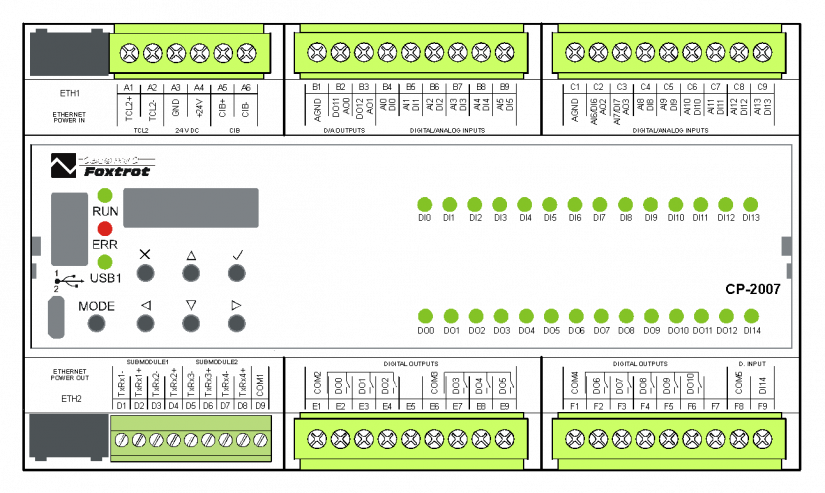
\includegraphics[scale=0.7]{obrazky/CP-2007.png}
    \end{center}
    \caption[CP-2007 \cite{TECO}]{CP-2007 \cite{TECO}}
    \label{fig:CP-2007}
\end{figure}

\section{Mosaic}
Ovládání instalace bylo realizováno v programovacím prostředí společnosti TECO - Mosaic, které je určeno pro programování PLC. Toto prostředí nabízí široké spektrum funkcí a nástrojů pro programování, vizualizaci a správu projektů \cite{Mosaic}: 

\begin{itemize}
    \item \textbf{Programovací jazyky dle IEC 61131-3 \cite{IEC61131-3}:}
        \begin{itemize}
            \item Ladder Diagram (LD)
            \item Function Block Diagram (FBD)
            \item Structured Text (ST)
            \item Instruction List (IL)
            \item Sequential Function Chart (SFC)
            \item Continuous Function Chart (CFC)
        \end{itemize}
    \item \textbf{Simulační nástroje:}
        \begin{itemize}
            \item Simulátor PLC
            \item Simulátor panelu
        \end{itemize}
    \item \textbf{Archivační nástroje:}
        \begin{itemize}
            \item Datalogger
            \item Správce souborů projektu
            \item Správce knihoven
        \end{itemize}
    \item \textbf{Nástroje pro tvorbu vizualizace:}
        \begin{itemize}
            \item WebMaker
            \item PanelMaker
            \item GraphMaker
        \end{itemize}
    \item \textbf{Inženýrské a pomocné nástroje:}
        \begin{itemize}
        \item Mapování uživatelských registrů
        \item I/O konfigurátor
        \item PID Maker
        \item PLCnet Manažer
        \item LangMan (jazykový manažer)
        \item Debuger
        \item IEC Manažer
        \item Asistent 16 → 32 (Převod 16bitového projektu na 32bitový)
        \item Texty KEY2 (Správa textových řetězců pro operační panely KEY2)
        \item Import KNX (Import konfigurace KNX/IP BAOS z csv souboru)
        \item Firmware Updater
        \item Project Loader
        \item Set PLC IP
        \item Mosaic Updater
        \item Jazyk prostředí / IDE Language
    \end{itemize}
\end{itemize}

\subsection{Ovládací prvky}
Pro ovládání instalace byly vytvořeny funkční bloky, které byly poté použity v realizaci logiky programu:

\begin{itemize}
    \item \textbf{Základní funkční bloky:}
        \begin{itemize}
            \item fbKNXVisuBool - Ovládání binárních signálů skrze vizualizaci
            \item fbKNXShutters - Ovládání žaluzií skrze vizualizaci
            \item fbRoomTempMod - Modelovaní teploty místnosti v závislosti na parametrech a vstupech z topení a klimatizace (měření teploty z panelu bude neměnné - neumožní demonstraci změny teploty)
        \end{itemize}
    \item \textbf{Funkční bloky jednotlivých místností:}
        \begin{itemize}
            \item fbLivRoom - Ovládání obývacího pokoje a simulace teploty
            \item fbKitch - Ovládání kuchyně a simulace teploty
            \item fbBath - Ovládání koupelny a simulace teploty
            \item fbOutz - Ovládání vstupu a měření venkovní teploty (teplota z panelu) \newline
        \end{itemize}
\end{itemize}

\noindent Níže jsou uvedeny definice jednotlivých funkční bloků, které byly použity pro ovládání a vizualizaci instalace. Pro jejich realizaci byly použity jazyky CFC a ST.

\subsubsection{fbKNXVisuBool}
\begin{lstlisting}[language=ST, breaklines=true, numbers=left, numberstyle=\small, numbersep=10pt, frame=single, basicstyle=\ttfamily\small, caption={Definice funkčního bloku fbKNXVisuBool}, label={lst:fbKNXVisuBool}]
FUNCTION_BLOCK fbKNXVisuBool
  VAR_INPUT
    IN           : BOOL R_EDGE; //Světlo ON Vizu
    OFF          : BOOL R_EDGE; //Světlo OFF Vizu
    FB           : BOOL; //KNX Světlo Feedback
  END_VAR
  VAR_OUTPUT
    OUT_CMD      : DT_CMD_BOOL; //KNX CMD
    OUT          : BOOL; //Visu hodnota
  END_VAR
  VAR
    TP_TIME : TIME := T#1S; //KNX CMD délka
    RS1 : RS;
    TP1 : TP;
  END_VAR

\end{lstlisting}

\begin{figure}[!ht]
    \begin{center}
        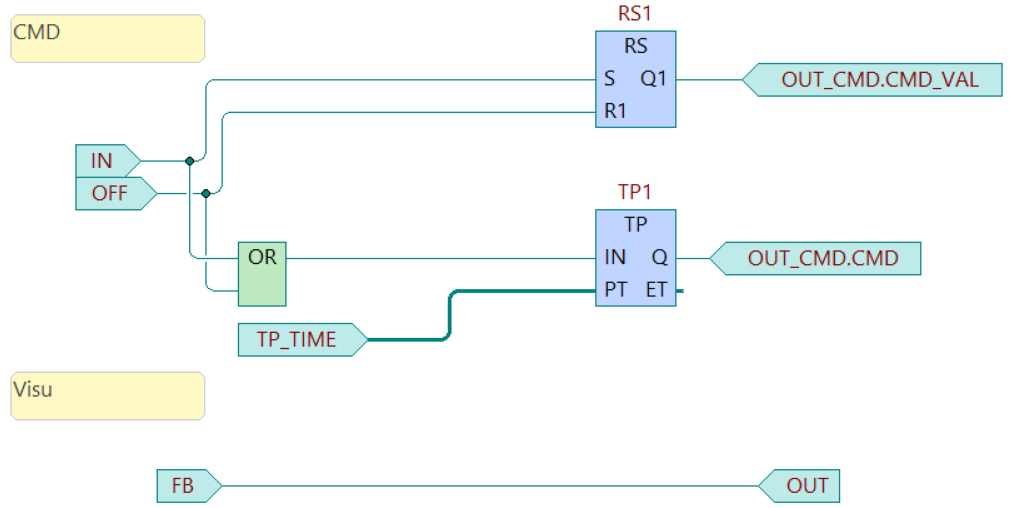
\includegraphics[scale=0.5]{obrazky/fbKNXVisuBool.png}
    \end{center}
    \caption[fbKNXVisuBool]{fbKNXVisuBool}
    \label{fig:fbKNXVisuBool}
\end{figure}
\newpage
\subsubsection{fbKNXShutters}
\begin{lstlisting}[language=ST, breaklines=true, numbers=left, numberstyle=\small, numbersep=10pt, frame=single, basicstyle=\ttfamily\small, caption={Definice funkčního bloku fbKNXShutters}, label={lst:fbKNXShutters}]
    FUNCTION_BLOCK fbKNXShutters
    VAR_INPUT
      UP           : BOOL R_EDGE; //Rolety nahoru Vizu
      DOWN         : BOOL R_EDGE; //Rolety dolu Vizu
      UP_STEP      : BOOL; //Rolety nahoru krok Vizu
      DOWN_STEP    : BOOL; //Rolety dolu krok Vizu
      FB_UP        : BOOL; //KNX Rolety Feedback nahoru
      FB_DOWN      : BOOL; //KNX Rolety Feedback dolu
    END_VAR
    VAR_OUTPUT
      OUT_CMD      : DT_CMD_BOOL; //KNX CMD
      OUT_STEP_CMD : DT_CMD_BOOL; //KNX CMD krok
      OUT_UP       : BOOL; //Visu nahoru
      OUT_DOWN     : BOOL; //Visu dolu
    END_VAR
    VAR
      TP_TIME : TIME := T#1S; //KNX CMD délka
      RS1 : RS;
      TP1 : TP;
      RS2 : RS;
    END_VAR
\end{lstlisting}

\begin{figure}[!ht]
    \begin{center}
        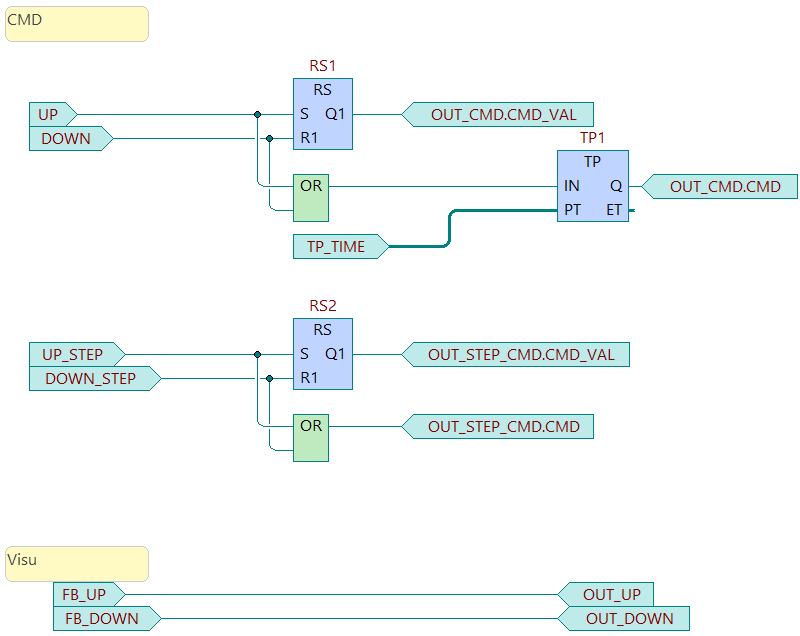
\includegraphics[scale=0.7]{obrazky/fbKNXShutters.png}
    \end{center}
    \caption[fbKNXShutters]{fbKNXShutters}
    \label{fig:fbKNXShutters}
\end{figure}
\subsubsection{fbRoomTempMod}
Na modelování teploty místnosti byl vytvořen jednoduchý matematický model, který měl za úkol zobrazit změnu v závislosti na působení topení a klimatizace. Uvažujeme, že místnost je kvádr o rozměrech specifikovaných uživatelským vstupem. Tento kvádr je naplněný vzduchem, který má určitou váhu, ze které lze vypočítat energii potřebnou ke změně teploty o 1 °C.

\begin{equation}
    V = a \cdot b \cdot c
    \label{eq:objem}
\end{equation}
\begin{equation}
    m = \rho \cdot V
    \label{eq:hmotnost}
\end{equation}
\begin{equation}
    Q = m \cdot c_p
    \label{eq:energie}
\end{equation}
\noindent\textit{Kde:}
\begin{itemize}
    \item $V$ -- objem vzduchu v místnosti [m$^3$]
    \item $a$, $b$, $c$ -- rozměry místnosti [m]
    \item $m$ -- hmotnost vzduchu v místnosti [kg]
    \item $\rho$ -- hustota vzduchu při tlaku jedné atmosféry a teplotě 20 °C - 1.204 [kg/m$^3$]
    \item $Q$ -- energie potřebná ke změně teploty o 1 stupeň teploty [J]
    \item $c_p$ -- měrná tepelná kapacita vzduchu - 1005 [J$\cdot$kg$^{-1}\cdot$K$^{-1}$] \newline
\end{itemize}
\noindent Dále uvažujeme obal kvádru (stěny, podlahu a strop) s různými tloušťkami a tepelnými vodivostmi (Fourierův zákon vedení tepla \ref{eq:tepelny_tok}). Pro zjednodušení výpočtu se předpokládá, že dveře a okna místnosti nemají rozdílný vliv oproti stěnám, tudíž tepelný tok zůstává na celé ploše strany stejný. Zároveň směr toku závisí pouze na poměru teplot na obou stranách zdi. Dále je předpoklad nulových teplot z jiných směrů. Také budeme předpokládat, že materiál bude všude stejný a to pálená cihla. 

\begin{equation}
    S = a \cdot b
    \label{eq:plocha}
\end{equation}
\begin{equation}
    \Delta T = T_{in} - T_{out}
    \label{eq:rozdil_teplot}
\end{equation}
\begin{equation}
    \phi _{Strana} = \frac{\lambda \cdot S \cdot \Delta T}{c}
    \label{eq:tepelny_tok}
\end{equation}
\noindent\textit{Kde:}
\begin{itemize}
    \item $S$ -- plocha strany [m$^2$]
    \item $a$, $b$, $c$ -- rozměry strany [m]
    \item $\Delta T$ -- rozdíl teploty na obou stranách strany [°C]
    \item $T_{in}$ -- teplota uvnitř místnosti [°C]
    \item $T_{out}$ -- teplota venku [°C]
    \item $\phi _{Strana}$ -- tepelný tok [W]
    \item $\lambda$ -- tepelná vodivost cihly - 0.4 [W$\cdot$m$^{-1}\cdot$K$^{-1}$] \newline
\end{itemize}
\noindent Další součástí simulace je topení a klimatizace, které jsou dodávány pouze jako binární signály. Pro jednoduché modelování byly vytvořeny funkce růstu (logaritmický) a poklesu (exponenciální) výkonu. Tyto funkce jsou zobrazeny na Obr. \ref{fig:simulace_funkce} Dále byly k těmto rovnicím vytvořeny korekční členy, které ovlivňují rychlost funkcí, a tedy více přiblížily chování funkcí realitě.

\begin{equation}
    f_{Růst}(t) = \frac{ln(1 + k_{Růst} \cdot t)}{ln(1 + k_{Růst} \cdot t_{MaxRůst})} \cdot y_{Max}
    \label{eq:funkce_rust}
\end{equation} 
\begin{equation}
    k_{Růst} = \frac{t_{MaxRise}}{t_{80}}
    \label{eq:k_rust}
\end{equation}
\begin{equation}
    f_{Pokles}(t) = \frac{y}{e^{k_{Pokles} \cdot t}}
    \label{eq:funkce_pokles}
\end{equation}
\begin{equation}
    k_{Pokles} = \frac{\frac{y_{max}}{\varepsilon}}{t_{MaxPokles}}
    \label{eq:k_pokles}
\end{equation}
\newpage
\noindent\textit{Kde:}
\begin{itemize}
    \item $f_{Růst}(x)$ -- funkce růstu výkonu [W]
    \item $k_{Růst}$ -- korekční člen pro pokles [-]
    \item $t$ -- čas [s]
    \item $t_{MaxRůst}$ -- maximální čas růstu výkonu [s]
    \item $y_{Max}$ -- maximální výkon [W]
    \item $t_{80}$ -- čas potřebný k dosažení 80\% výkonu [s]
    \item $f_{Pokles}(x)$ -- funkce poklesu výkonu [W]
    \item $k_{Pokles}$ -- korekční člen pro růst [-] 
    \item $y$ -- aktuální výkon [W]
    \item $\varepsilon$ -- cílová hodnota, pod kterou se výkon musí dostat [W]
    \item $t_{MaxPokles}$ -- maximální čas poklesu výkonu [s]
\end{itemize}
\begin{figure}[!ht]
    \begin{center}
        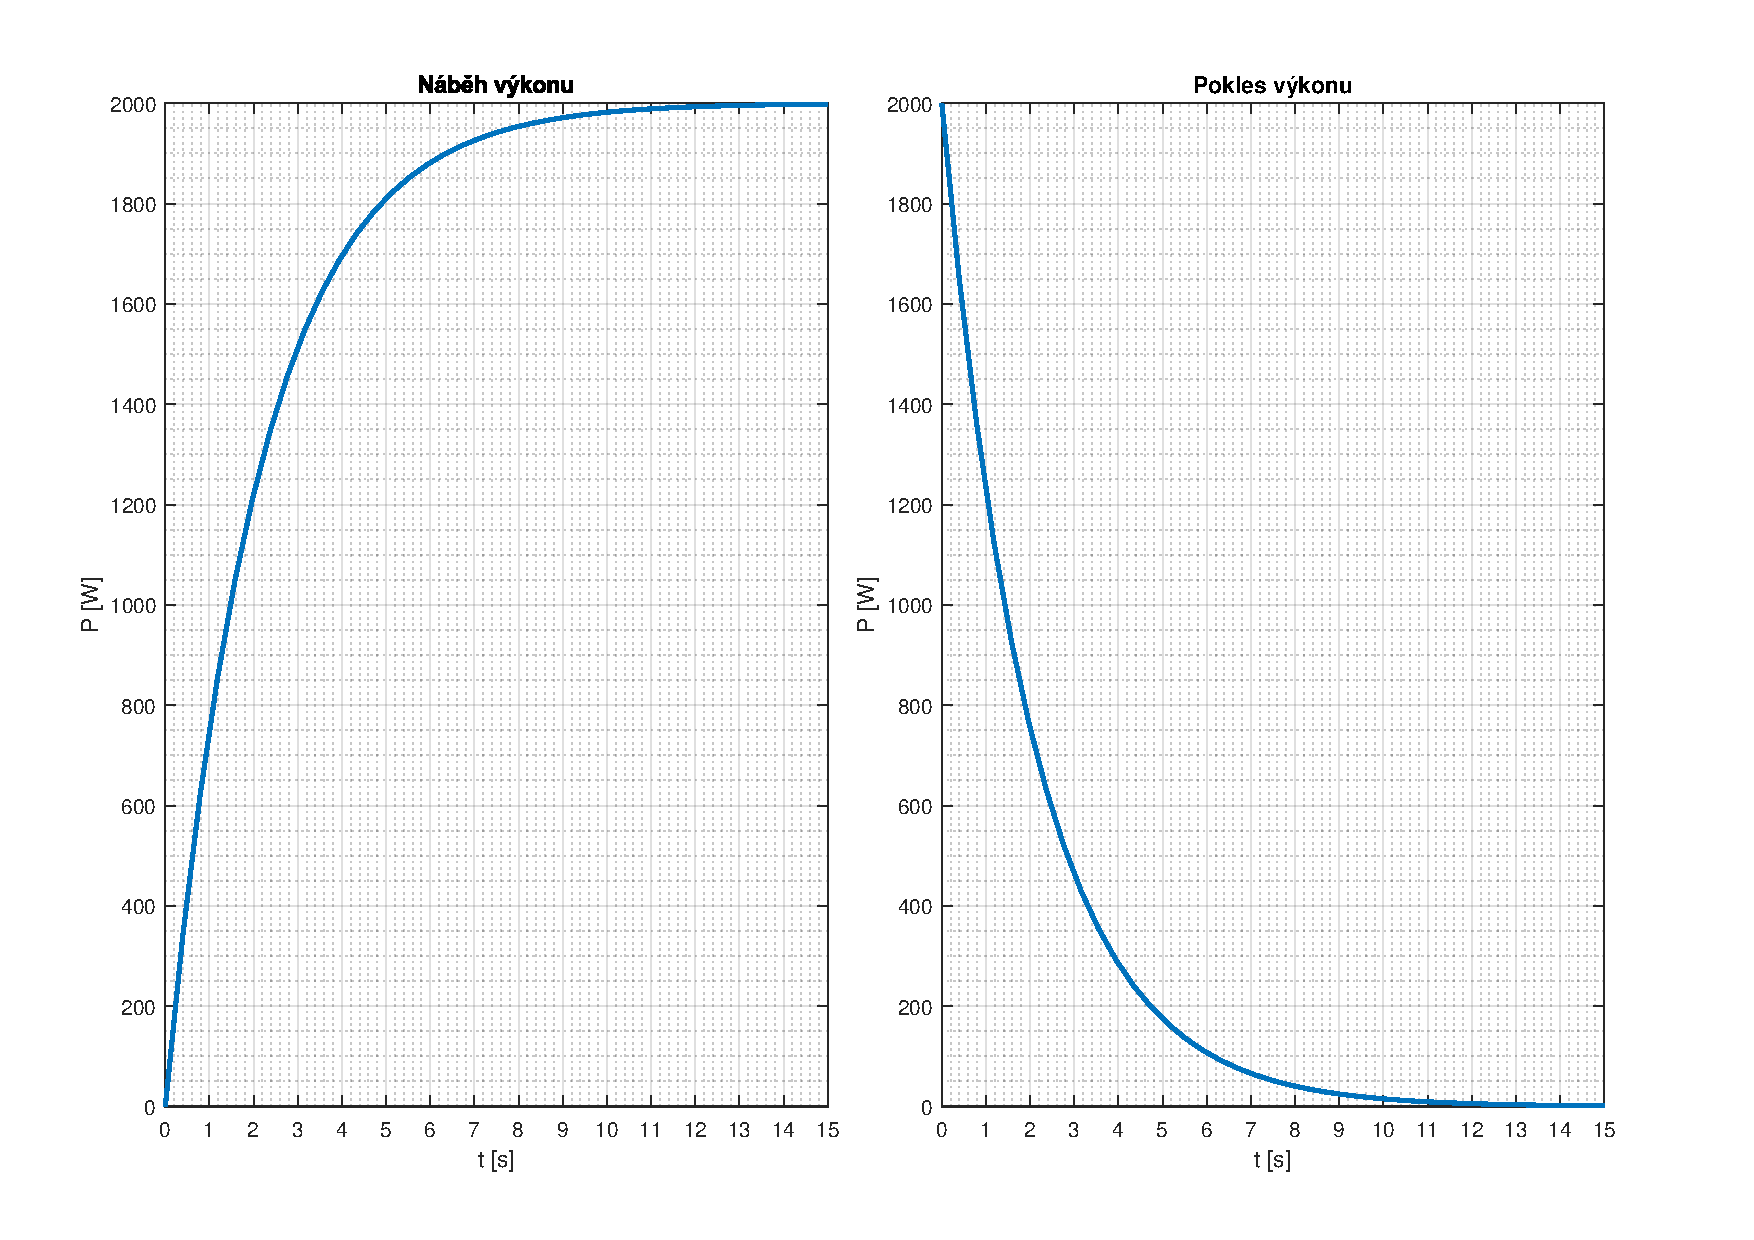
\includegraphics[scale=0.52]{obrazky/simulace_funkce.pdf}
    \end{center}
    \caption[Průběh funkcí pro simulaci]{Průběh funkcí pro simulaci}
    \label{fig:simulace_funkce}
\end{figure}
\noindent Tyto funkce bylo potřeba převést do rekurzivní podoby, aby bylo možné je implementovat do funkčního bloku.
\begin{equation}
    y_{RůstTed} = y_{RůstPred} + \frac{ln(1 + k_{Růst} \cdot \Delta t)}{ln(1 + k_{Růst} \cdot T_{Max})} \cdot (y_{Max} - y_{RůstPred}) 
    \label{eq:rust_rekurzivni}
\end{equation}
\begin{equation}
    y_{PoklesTed} = y_{PoklesPred} \cdot e^{k_{Pokles} \cdot \Delta t}
    \label{eq:pokles_rekurzivni}
\end{equation}
\noindent\textit{Kde:}
\begin{itemize}
    \item $y_{RůstTed}$ -- nový výkon [W]
    \item $y_{RůstPred}$ -- předchozí výkon [W]
    \item $k_{Růst}$ -- korekční člen pro pokles [-]
    \item $\Delta t$ -- časový krok [s]
    \item $T_{Max}$ --maximální čas růstu výkonu [s]
    \item $y_{Max}$ -- maximální výkon [W]
    \item $y_{PoklesTed}$ -- nový výkon [W]
    \item $y_{PoklesPred}$ -- předchozí výkon [W] \newline
\end{itemize}
\noindent Po vyčtení výkonu topení a klimatizace zbývá vypočítat teplotu v místnosti. Ta se získá součtem aktuální hodnoty teploty, přírůstku podílu působících toků a potřebné energie ke změně teploty. (Rov. \ref{eq:energie}). Rovnice pro celkový tepelný tok je dána jako součet tepelných toků ze stran, výkonu topení a klimatizace (působí záporně).
\begin{equation}
    T_{Aktualni} = T_{Predchozi} + \frac{\phi _{Celkovy} \cdot \Delta t}{Q}
    \label{eq:aktualni_teplota}
\end{equation}
\begin{equation}
    \phi _{Celkovy} = \sum_{i=1}^{6} \phi _{Strana_i} + \phi _{Topeni} - \phi _{Klimatizace}
    \label{eq:celkovy_tepelny_tok}
\end{equation}
\noindent\textit{Kde:}
\begin{itemize}
    \item $T_{Aktualni}$ -- aktuální teplota [°C]
    \item $T_{Predchozi}$ -- předchozí teplota [°C]
    \item $\Delta t$ -- časový krok [s]
    \item $\phi _{Celkovy}$ -- celkový tepelný tok [W]
    \item $\phi _{Strana_i}$ -- tepelný tok ze strany \textit{i} [W]
    \item $\phi _{Topeni}$ -- tepelný tok z topení [W]
    \item $\phi _{Klimatizace}$ -- tepelný tok z klimatizace [W] \newline
\end{itemize}

\noindent Průběh teploty v místnosti je zobrazen na Obr. \ref{fig:simulace_teplota}, kde je demonstrováno chování při běhu topení a klimatizace v horním grafu. Ve spodní části grafu je zase zobrazeno chování teploty bez působení topení a klimatizace. Teplota okolí je v tomto případě nastavená na 21 °C. Z průběhu lze vypozorovat, že se teplota ustálí na teplotu okolí a tudíž, lze považovat model za korektní.
\newpage
\begin{figure}[!ht]
    \begin{center}
        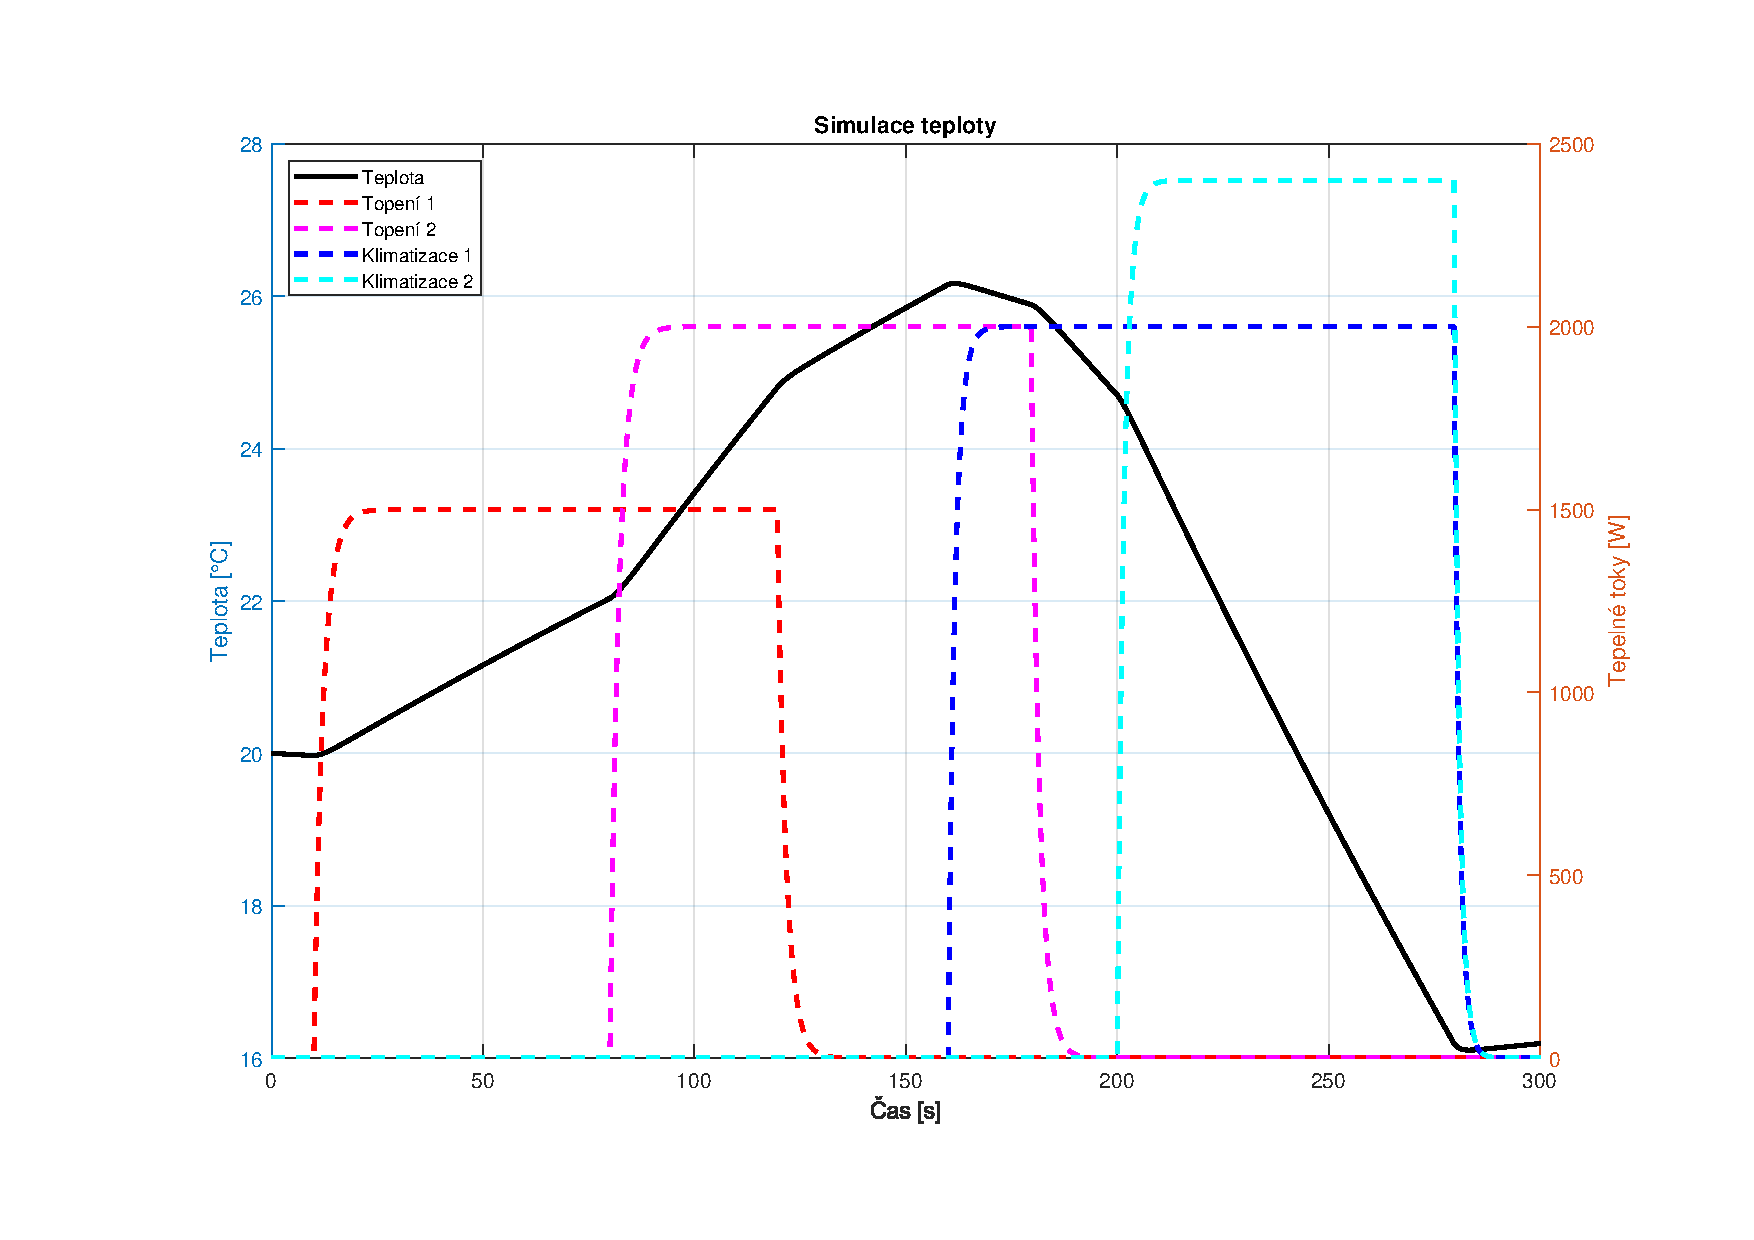
\includegraphics[scale=0.52]{obrazky/simulace_teploty_kuchyne.pdf}
    \end{center}
    \caption[Simulace teploty v místnosti]{Simulace teploty v místnosti}
    \label{fig:simulace_teplota}
\end{figure}

\noindent Tento funkční blok byl použit pro simulaci teploty v obývacím pokoji, kuchyni. Definice tohoto funkčního bloku je zobrazena kvůli své velikosti v příloze \ref{apend:fbRoomTempMod}. Pro venkovní teplotu byl použit signál, který byl napojen na teploměr na panelu. V případě koupelny byla teplota simulována jako sinusoida v rozmezí 18-22 °C s periodou 3 minuty. Tento způsob byl zvolen kvůli absenci teploměru a akčního členu pro řízení teploty. 

\subsubsection{funkční bloky jednotlivých místností}
\label{subsection:fb_mistnosti}
Funkční bloky jednotlivých místností se skládají z výše uvedených funkcí, které byly poskládány v závislosti na požadavcích jednotlivých místností - viz Obr. \ref{fig:Vzheled panelu}. Všechny funkční bloky mají definici vypsanou v přílohách dokumentu:
\begin{itemize}
    \item \textbf{fbBath} - V příloze \ref{apend:fbBath}
    \item \textbf{fbKitch} - V příloze \ref{apend:fbKitch}
    \item \textbf{fbLivRoom} - V příloze \ref{apend:fbLivRoom}
    \item \textbf{fbOutz} - V příloze \ref{apend:fbOutz}
\end{itemize}
\subsection{Komunikace KNX/IP}
Důležitou součástí ovládání instalace je komunikace s KNX/IP, která byla realizována pomocí knihovny KNXlib \cite{KNXlib}. Obsahem této knihovny jsou dva funkční bloky určené ke komunikaci:
\begin{itemize}
    \item \textbf{fbKnxIpBaos} - Funkční blok pro komunikaci s KNX/IP BAOS 772 v režimu TCP master
    \item  \textbf{fbKnxIpBaosBin} - Funkční blok pro komunikaci s KNX/IP BAOS 772/774 skrze binární protokol v režimu TCP Master \newline
\end{itemize}
Dále tato knihovna obsahuje datové struktury, které obsahují definice jednotlicých datapointů, které jsou potřeba pro komunikaci mezi PLC a KNX/IP Baos 774:
\begin{table}[h]
    \caption[Definice KNX datapointů v PLC]{Definice KNX datapointů v PLC}
        \small
            \centering
            \begin{tabular}{|c|c|c|}
                \hline
                Typ objektu KNX & Datový typ PLC & Popis  \\
                \hline\hline
                DPT 01 & T\_KNX\_OBJECT\_DPT1 & Binární signál -- 1 Bit \\
                \hline
                DPT 02 & T\_KNX\_OBJECT\_DPT2 & Binární signál s kontrolou (Priorita) -- 2 Bity \\
                \hline
                DPT 03 & T\_KNX\_OBJECT\_DPT3 & Stmívání nahoru/dolů -- 4 Bit \\
                \hline
                DPT 04 & T\_KNX\_OBJECT\_DPT4 & Znak -- 1 bajt \\
                \hline
                DPT 05 & T\_KNX\_OBJECT\_DPT5 & Škálování -- 1 bajt (8 Bitová hodnota) \\
                \hline
                DPT 06 & T\_KNX\_OBJECT\_DPT6 & Hodnota se znaménkem -- 1 bajt \\
                \hline
                DPT 07 & T\_KNX\_OBJECT\_DPT7 & Hodnota bez znaménka -- 2 bajty \\
                \hline
                DPT 08 & T\_KNX\_OBJECT\_DPT8 & Hodnota se znaménkem -- 2 bajty \\
                \hline
                DPT 09 & T\_KNX\_OBJECT\_DPT9 & Hodnota s desetinnou čárkou -- 2 bajty\\
                \hline
                DPT 10 & T\_KNX\_OBJECT\_DPT10 & Čas -- 3 bajty \\
                \hline
                DPT 11 & T\_KNX\_OBJECT\_DPT11 & Datum -- 3 bajty \\
                \hline
                DPT 12 & T\_KNX\_OBJECT\_DPT12 & Hodnota bez znaménka -- 4 bajty \\
                \hline
                DPT 13 & T\_KNX\_OBJECT\_DPT13 & Hodnota se znaménkem -- 4 bajty \\
                \hline
                DPT 14 & T\_KNX\_OBJECT\_DPT14 & Hodnota s desetinnou čárkou -- 4 bajty \\
                \hline
                DPT 15 & T\_KNX\_OBJECT\_DPT15 & Přístupová data -- 4 bajty \\
                \hline
                DPT 16 & T\_KNX\_OBJECT\_DPT16 & Řetězec znaků -- 14 bajty \\
                \hline
                DPT 17 & T\_KNX\_OBJECT\_DPT17 & Scéna -- 1 bajt \\
                \hline
                DPT 18 & T\_KNX\_OBJECT\_DPT18 & Kontroler scén -- 1 bajt \\
                \hline
                DPT unknown & T\_KNX\_OBJECT\_RAW & Max. 14 bajtů, Data jako pole, byte-by-byte \\
                \hline
            \end{tabular}
\end{table}
\subsubsection{Realizace komunikace KNX/IP}
Pro realizaci v tomto případě bylo potřeba kromě přidání knihovny a vytvoření programu ještě i nastavit ethernet port. V tomto případě byl do \textit{ETH2} přidán obecný kanál \textit{UNI1}, který bylo potřeba nastavit jako TCP Server. Dále je pak nutné vytvořit několik proměnných dle tabulky datapointů \ref{tab:Datapointy pro komunikaci KNX IP BAOS 774 s PLC}, získat jejich adresy a poté je vložit do pole.

Dalším krokem je nastavení funkčního bloku \textit{fbKnxIpBaosBin}. Nejprve se nastaví číslo prvního a posledního datapointu, který má funkční blok zpracovat, poté se nastaví použitý ethernet port a IP adresa KNX/IP BAOS 774 instalace. Nakonec se předá do portu \textit{knxList} námi definované pole s adresami. Po tomto kroku je už možné pracovat s proměnnými a vytvoření ovládací logiku.

V případě této práce se používají pouze 3 druhy datapointů a to:
\begin{itemize}
    \item \textbf{DPT 1} - ovládání a indikace binárního signálu
    \item \textbf{DPT 9} - hodnota teploty z teploměru
    \item \textbf{DPT 18} - ovládání scény \newline
\end{itemize}
Níže je uvedena ukázka realizace komunikace, která vyplývá z implementace uvedené v příloze \ref{apend:KNXComm}:
\begin{lstlisting}[language=ST, breaklines=true, numbers=left, numberstyle=\small, numbersep=10pt, frame=single, basicstyle=\ttfamily\small, caption={Implementace komunikace KNX/IP}, label={lst:komunikace_knx}]
PROGRAM prgKNXComm
  VAR
    init : BOOL;
    knx  : fbKnxIpBaosBin;
    knxObjectList    : ARRAY[1..4] OF UDINT; // pole adres
    datapoint1      : T_KNX_OBJECT_DPT1;     // SV1_FB
    datapoint2      : T_KNX_OBJECT_DPT1;     // SV1_CMD
    datapoint3      : T_KNX_OBJECT_DPT18;    // scéna
    datapoint4      : T_KNX_OBJECT_DPT9;     // teplota
  END_VAR

IF NOT init THEN // Pole adres
  knxObjectList[1]  := PTR_TO_UDINT( ADR(datapoint1));
  knxObjectList[2]  := PTR_TO_UDINT( ADR(datapoint2));
  knxObjectList[3]  := PTR_TO_UDINT( ADR(datapoint3));
  knxObjectList[4]  := PTR_TO_UDINT( ADR(datapoint4));
  init := TRUE;
END_IF

knx( firstKnxObject := 1,
     lastKnxObject := 4,
     ethCode := ETH2_uni2,
     knxIP := STRING_TO_IPADR('192.168.xxx.xxx'),
     knxList := void( knxObjectList));
\end{lstlisting}
\begin{lstlisting}[language=ST, breaklines=true, firstnumber=25, numbers=left, numberstyle=\small, numbersep=10pt, frame=single, basicstyle=\ttfamily\small]

SV1_FB := datapoint1.value; // Feedback
IF SV1_CMD THEN datapoint2.value := SV1_CMD.CMD_VAL; // CMD

IF SCENE THEN // scéna
  datapoint3.control := TRUE;
  datapoint3.scene   := 5;
END_IF

KNX_TEMPER := datapoint4.value;// Posílání teploty
END_PROGRAM
\end{lstlisting}
\subsection{Komunikace MQTT}
\label{subsection:MQTT}
Tato sekce je zaměřená na realizaci komunikace skrze protokol MQTT, který je navržen jako lehký přenos zpráv mezi zařízeními a aplikacemi. Jeho cílovou skupinou jsou zařízení s malou kódovou stopou a minimální šířkou pásma sítě. \cite{MQTT}

\subsubsection{Protokol}
Základními myšlenkami protokolu MQTT je posílání zpráv mezi vydavatelem (publisher) a odběratelem(client) skrze zprostředkovatele (broker). Tento broker zajišťuje, že zprávy jsou doručeny správným odběratelům. Vydavatel a odběratel nemusí být navzájem známi a komunikují pouze skrze brokera. \cite{MQTT}

Tento druh komunikace je realizován pomocí packetů (balíků dat) posílaných mezi zařízeními. Jednotlivé datové balíky jsou tvořen třemi částmi \cite{MQTTEsentials}:
\begin{itemize}
    \item \textbf{Fixní hlavičku} - obsahuje informace o typu packetu, příznaky a velikost zbylé části packetu 
    \item \textbf{Volitelnou hlavičku} - obsahuje dynamické informace o packetu
    \item \textbf{Datový obsah} - obsahuje data, která se posílají mezi zařízeními \newline
\end{itemize}
Zprávy se poté posílají na určité téma (topic), které je definováno jako hierarchická struktura. Tato struktura je tvořena jednotlivými úrovněmi oddělenými lomítkem. V případě této práce je dobrým příkladem téma \textit{plc/Connect/Publisher}, kde:
\begin{itemize}
    \item \textbf{plc} - označuje zařízení, které zprávu odesílá
    \item \textbf{Connect} - která část systému zprávu odesílá
    \item \textbf{Publisher} - bližší rozlišení \newline
\end{itemize}
Dálší část je text samotné zprávy, která je odeslána na dané téma. Tato zpráva může mít libovolnou strukturu i velikost(maximálně 256 MB). Tělem zprávy je text ve formátu JSON, který se lze pochopit jako hierarchická struktura dat. Vertikálně je struktura rozdělena do úrovní pomocí vnořených objektů a polí. Horizontálně je struktura členěna do jednotlivých klíč:hodnota párů na jedné úrovni, kde každý klíč reprezentuje konkrétní parametr. Příkladem takové zprávy je:
\begin{lstlisting}[language=JSON, breaklines=true, numbers=left, numberstyle=\small, numbersep=10pt, frame=single, basicstyle=\ttfamily\small, caption={Příklad zprávy v JSON}, label={lst:json}]
{
    "device": "plc",
    "location": {
        "room": "kitchen",
        "floor": 1
    },
    "sensors": {
        "temperature": {
            "value": 22.5,
            "unit": "C"
        },
        "humidity": {
            "value": 45,
            "unit": "%"
        }
    },
    "status": "online",
    "timestamp": "2024-06-01T12:34:56Z"
}
\end{lstlisting}

\noindent Součástí zprávy je i kvalita služeb \textit{QoS} (Quality of Service), která určuje úroveň spolehlivosti doručení zprávy. Tato úroveň je nastavena na 0 (doručení maximálně jednou bez záruky), 1(doručená alespoň jednou) nebo 2(doručená přesně jednou s potvrzením příjemce) \cite{MQTTEsentials}. V případě této práce byla zvolena úroveň QoS 1, která je dostatečná pro většinu aplikací a poskytuje dobrou rovnováhu mezi spolehlivostí a výkonem. 

Poslední součástí zprávy je \textit{Last Will and Testament} (LWT), což je zpráva, která je odeslána brokerem v případě, že se zařízení odpojí bez předchozího oznámení. Tato zpráva může být užitečná pro monitorování stavu zařízení a detekci výpadků \cite{MQTTEssentials}.

\subsubsection{MQTTlib}
Pro realizaci komunikace mezi PLC a Home Assistantem byla použita knihovna MQTTlib, která obsahuje funkční bloky pro nastolení komunikace - \textit{fbMQTTPublisher}, \textit{fbMQTTSubscriber}. \cite{MQTTlib}

Prvním krokem pro realizaci komunikace je nastavení ethernet portu, který bude použit pro komunikaci. V případě této práce byl použit stejný port jako pro KNX/IP komunikaci (\textit{ETH2}). Na tomto portu byly vytvořeny dva obecné kanály \textit{UNI0} a \textit{UNI1}, které byly nastaveny jako TCP clienty s šíkou pásma 512 bytů. Počet kanálu závisí na počtu nastolených spojení. Pro jednoduchost se jedná o jedno spojení pro publikování a jedno pro odběr zpráv. 

Dalším krokem je nastavení funkčních bloků. V obou případech je nastavení obdobné. Nejprve se nastaví kanál na kterém bude komunikace probíhat - IP adresa brokeru, port brokeru, lokální port, časový interval pro kontrolu spojení a délku nečinosti. Dále se nastaví parametry komunikace a poslední vůle:
\begin{itemize}
    \item \textbf{clientID\_auto} - automatické generování identifikátoru klienta
    \item \textbf{clientID} - identifikátor klienta
    \item \textbf{loginName} - uživatelské jméno pro připojení k brokeru
    \item \textbf{loginPass} - heslo pro připojení k brokeru
    \item \textbf{retain} - určuje zda má být zpráva uchována na brokeru
    \item \textbf{QoS} - určuje úroveň kvality služeb
    \item \textbf{cleanSession} - určuje zda má broker uložit stav relace po výpadku
    \item \textbf{topic} - téma komunikace
    \item \textbf{mess} - zpráva komunikace
    \item \textbf{flag} - určuje zda má být poslední vůle odeslána v případě odpojení klienta bez předchozího oznámení \newline
\end{itemize}

Po nastavení funkčních bloků je potřeba definovat proměnné na uchovávání zpráv. Maximální délka zprávy je 256 znaků pro oba funkční bloky. Níže je uveden příklad nastavení komunikace pro publikování zprávy:
\begin{lstlisting}[language=ST, breaklines=true, numbers=left, numberstyle=\small, numbersep=10pt, frame=single, basicstyle=\ttfamily\small, caption={Příklad nastavení komunikace pro publikování zprávy}, label={lst:publikace}]
PROGRAM prgMQTTPub
    VAR
        mqttPub : fbMQTTPublisher;

        brokerIPaddr      : STRING := '192.168.xxx.xxx'; // IP adresa brokeru
        brokerPort        : UINT := 1883; // Port brokeru
        localPort         : UINT := 60000; // Lokalni port
        keepAlive         : BOOL  := TRUE; // Udrzeni spojeni po vypadku
        keepAliveInterval : TIME  := T#60s; // Konec spojeni bez dat
        pingInterval      : TIME  := T#10s; // Kontrola spojeni
\end{lstlisting}
\begin{lstlisting}[language=ST, breaklines=true, firstnumber=11, numbers=left, numberstyle=\small, numbersep=10pt, frame=single, basicstyle=\ttfamily\small]
        connTimeOut       : TIME  := T#5s; // Maximalni delka odezvy

        pubComParam   : T_MQTT_COM_PUB_PARAM := (
        pRetain := TRUE, // Uchovani zpravy na brokeru
        qos     := 1, // Kvalita sluzeb
        dup     := FALSE, // Opakovani zpravy
        clean   := FALSE // Uchovani stavu relace
        );

        willParamPub  : T_MQTT_COM_WILL_PARAM := (
        wRetain := FALSE, // Uchovani posledni vule na brokeru
        topic   := 'plc/Connect/Publisher', // Tema poslední vule
        mess    := 'Disconnected', // Zprava posledni vule
        flag    := TRUE, // Odeslani posledni vule
        qos     := 1 // Kvalita sluzeb
        );

        jsonPayload : STRING[255]; // Zprava
        topic      : STRING[80] := 'plc/test'; // Tema
    END_VAR

jsonPayload := CONCAT(
    '{',"test",'}'
);
mqttPub(
    chanCode          := ETH2_uni1, // Fyzicky kanal
    brokerIP          := STRING_TO_IPADR(brokerIPaddr),
    brokerPort        := brokerPort,
    localPort         := localPort,
    connect           := TRUE, // Pripojit k brokeru
    keepAlive         := keepAlive,
    keepAliveInterval := keepAliveInterval,
    pingInterval      := pingInterval,
    connTimeOut       := connTimeOut,
    clientId_auto     := FALSE, // Automaticke generovani ID
    clientId          := 'TEST_PUB', // ID klienta
    comParam          := pubComParam, // Parametry komunikace
    willParam         := willParamPub, // Parametry posledni vule
    topicTxt          := topic, // Tema
\end{lstlisting}
\pagebreak
\begin{lstlisting}[language=ST, breaklines=true, firstnumber=50, numbers=left, numberstyle=\small, numbersep=10pt, frame=single, basicstyle=\ttfamily\small]
    dataTxt           := jsonPayload, // Zprava
    sendCom           := TRUE // Odeslani zpravy
);
END_PROGRAM
\end{lstlisting}

Implementace použitá v této práci je uvedena v příloze \ref{apend:MQTTComm}. Jedná se o nastavení komunikace pro komunikaci s Home Assistantem, který přijímá hodnoty teplot místností a odesílá příkaz pro celkové vypnutí instalace. 
\subsection{Vizualizace}
V této sekci je popsána tvorba vizualizace panelu pomocí integrovaného webového serveru. Nastavení a realizace webového serveru je realizována pomocí integrovaného nástroje WebMaker. Tento nástroj je popsán v dokumentaci \cite{WebMaker}.

Prvním krokem je vytvoření struktury projektu. V tomto případě to bude 5 stránek ve formátu .XML zasazených do webové struktury: \newline

\dirtree{%
.1 /Vizualizace.
.2 Prehled - PAGE1.xml.
.2 Veranda - PAGE2.xml.
.2 Kuchyn - PAGE3.xml.
.2 Koupelna - PAGE4.xml.
.2 Obyvaci\_pokoj - PAGE5.xml. 
}
\vspace{0.3cm}
Druhým krokem bylo importování sady ikon, které byly použity jako vícerozměrné obrázky napojené na výstupy funkčních bloků uvedených v podkapitole \ref{subsection:fb_mistnosti}. Tyto ikony byly získány na stránce Flaticon \cite{Flaticon}, která poskytuje vektorové ikony na projekty zdarma s možností úpravy. 


\begin{figure}[!ht]
    \begin{center}
        
\includegraphics[scale=0.6]{obrazky/Ikonky.png}
    \end{center}
    \caption[Ikony použité pro vizualizaci]{Ikony použité pro vizualizaci}
    \label{fig:ikony}
\end{figure}

Dále se musely vytvořit ovládací tlačítka jednotlivých objektů. Tato tlačítka byla také vytvořena jako vícerozměrné obrázky, které byly napojeny na vstupy funkčních bloků. Pro zobrazování teplot v jednotlivých místnostech byla použita zadávací pole s parametrem \textit{Read only}. 
Výsledná vizualizace je uvedena v příloze \ref{apend:webmaker}. Vzhled byl zvolen minimalistický a funkční s ohledem na viditelnost a přehlednost. Černé pozadí zdůrazňuje kontrast ikon a textu. Dalším důvodem byla ochrana zraku při ovládání v noci.